\section{Software Ramp}

\subsection{Implementierung}\label{Appendix:Software_Ramp_Theorie}

In einer triangularen/trapezodialen Geschwindigkeits-Ramp ist die Bewegung in drei Phasen unterteilt. Die erste Phase besteht aus einer Beschleunigung in eine Richtung. Die Beschleunigung dauert so lange, bis das angetriebene Objekt die Maximalgeschwindigkeit erreicht. Sobald die Maximalgeschwindigkeit erreicht wurde, beginnt die zweite Phase. Während dieser Phase bewegt sich das Objekt mit konstanter Geschwindigkeit in die selbe Richtung wie die Beschleunigung. In der dritten Phase wird das Objekt wieder abgebremst mit einer Beschleunigung in die entgegengesetzte Richtung.

Die Formeln zur Berechnung der mechanischen Zustände sind für die Beschleunigung \ref{equ:Beschleunigung}, für die Geschwindigkeit \ref{equ:Geschwindigkeit} und für die Position \ref{equ:Position}. Je nach dem, in welche Richtung gefahren werden soll, wird das Vorzeichen der Beschleunigung geändert. Dafür wird beim FOC-Treiber die aktuelle Position abgefragt und berechnet, ob der Zielpunkt sich vor oder nach der aktuellen Position befindet.

\begin{equation}
a(t) = a_0
\label{equ:Beschleunigung}
\end{equation}

\begin{equation}
v(v) = v_0 + a_0 \cdot t
\label{equ:Geschwindigkeit}
\end{equation}

\begin{equation}
x(t) = x_0 + v_0 \cdot t + a_0 \cdot t ^ 2
\label{equ:Position}
\end{equation}

\begin{figure}[H]
\center
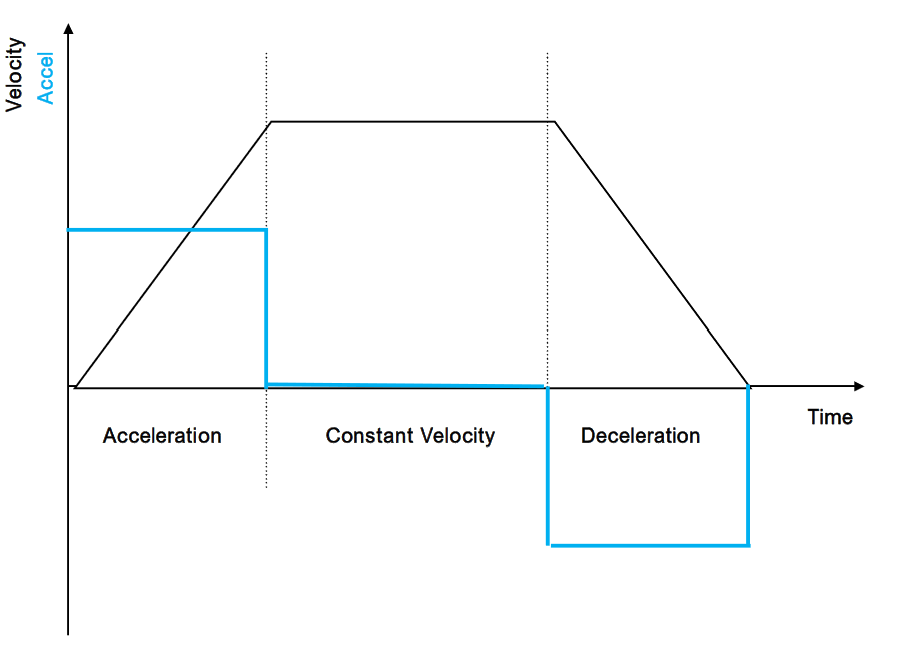
\includegraphics[width = 0.8 \textwidth]{graphics/Trapezodial_Ramp}
\caption{Trapezodiale Geschwindigkeits-Ramp. \cite{abb_application_2012}}
\label{fig:Trapezodial_Ramp}
\end{figure}

\begin{table}[H]
\center
\begin{tabular}{|l|l|l|l|}
\hline
Phase 				& $a_0$ 			& $v_0$ 			& $x_0$ 		\\
\hline
1 ($T_0 - T_1$)		& $+a_{max}$		& 0				& 0			\\
\hline
2 ($T_1 - T_2$)		& 0				& $v_{max}$		& x(t[n-1])	\\
\hline
3 ($T_2 - T_3$)		& $-a_{max}$		& $v_{max}$		& x(t[n-1])	\\
\hline
\end{tabular}
\caption{Parameter für trapezodiale Ramp.}
\end{table}

Eine weitere Möglichkeit, den Motor saft anlaufen zu lassen ist die S-Curve-Ramp. Diese besteht im Gegensatz zur trapezodialen Ramp statt aus drei Phasen aus sieben Phasen.

Die vier zusätzlichen Phasen kommen daher, dass jetzt die Beschleunigung nicht von Beginn weg voll anliegt, sondern auch linear hochgefahren wird. Die Zunahme der Beschleunigung wird auch Jerk genannt. \cite{collins_how_2017}

\begin{equation}
J(t) = J_0
\end{equation}

\begin{equation}
a(t) = a_0 + J_0 \cdot t
\label{equ:Beschleunigung_2}
\end{equation}

\begin{equation}
v(v) = v_0 + a_0 \cdot t + J_0 \cdot t^2
\label{equ:Geschwindigkeit_2}
\end{equation}

\begin{equation}
x(t) = x_0 + v_0 \cdot t + a_0 \cdot t ^ 2 + J_0 \cdot t^3
\label{equ:Position_2}
\end{equation}

\begin{figure}[H]
\center
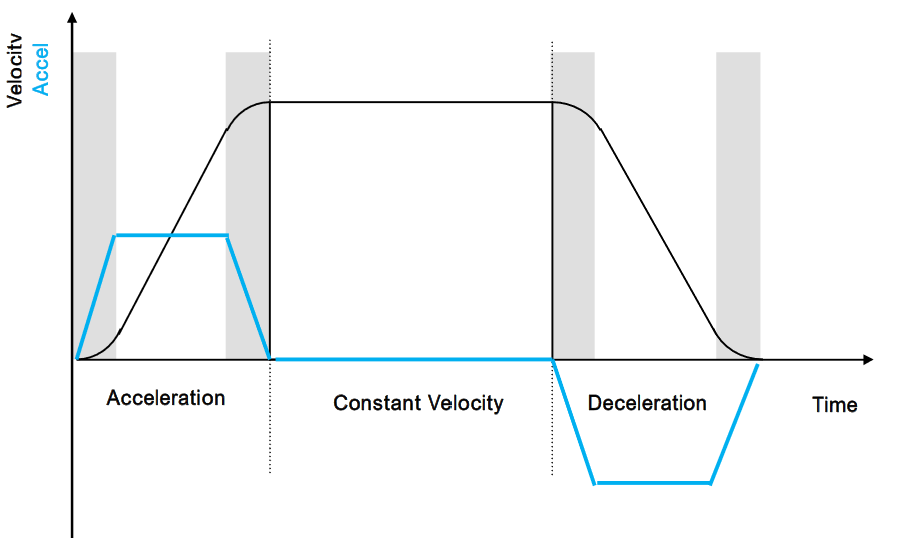
\includegraphics[width = 0.8 \textwidth]{graphics/S_Curved_Ramp}
\caption{S-Curve Geschwindigkeits-Ramp.\cite{abb_application_2012}}
\label{fig:S_Curved_Ramp_2}
\end{figure}

\begin{table}[H]
\center
\begin{tabular}{|l|l|l|l|l|}
\hline
Phase 				& 	$J_0$		& $a_0$ 			& $v_0$ 				& $x_0$ 				\\
\hline
1 ($T_0 - T_1$)		&	J			& 0				& 0					& 0					\\
\hline
2 ($T_1 - T_2$)		&	0			& a				& v$_{end Phase1}$	& x$_{end Phase1}$	\\
\hline
3 ($T_2 - T_3$)		&	-J			& a				& v$_{end Phase2}$	& x$_{end Phase2}$	\\
\hline
4 ($T_3 - T_4$)		&	0			& 0 				& v$_{end Phase3}$	& x$_{end Phase3}$	\\
\hline
5 ($T_4 - T_5$)		&	-J			& 0 				& v$_{end Phase4}$	& x$_{end Phase4}$	\\
\hline
6 ($T_5 - T_6$)		&	0			& -a				& v$_{end Phase5}$	& x$_{end Phase5}$	\\
\hline
7 ($T_6 - T_7$)		&	J			& -a				& v$_{end Phase6}$	& x$_{end Phase6}$	\\
\hline
\end{tabular}
\caption{Parameter für S-Curved Ramp.}
\end{table}

Die S-Curved-Ramp ist nicht implementiert und stellt einen Ansatz zur Verbesserung dar. Folgende Schritte können zu einer Implementierung führen:
\begin{itemize}
\item Strecke und Zeit messen für gesamten Beschleunigungsvorgang mit Jerk.
\item Daraus kann ermittelt werden, ob das zu bewegende Objekt schon über das Ziel herausschiesst.
\item Falls es darüber herausschiesst, muss der Beschleunigungsvorgang angepasst werden.
\item Der Vorgang erreicht die Höchstgeschwindigkeit dann nicht.
\item Danach kann der Algorithmus in die Software eingepasst werden.
\end{itemize}

\begin{figure}[H]
\center
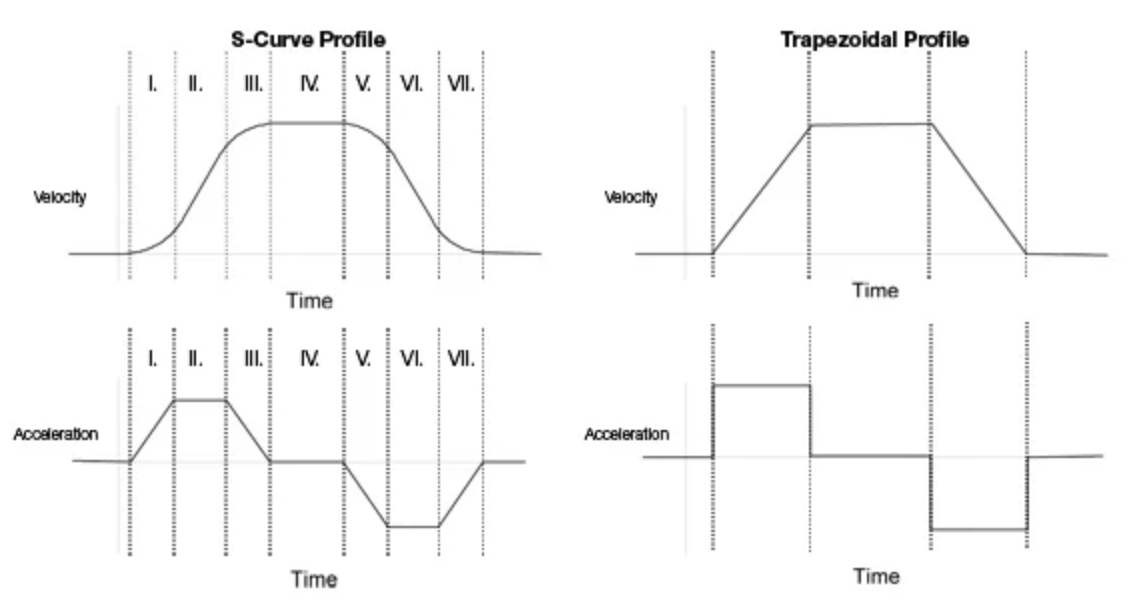
\includegraphics[width = \textwidth]{graphics/S_Curve_vs_trapezodial}
\caption{Vergleich S-Curve und trapezodial. \cite{lewin_s-curve_nodate}}
\label{fig:S_Curved_Ramp}
\end{figure}


\subsection{Matlab-Script}\label{Appendix:Ramp_Matlab_Script}

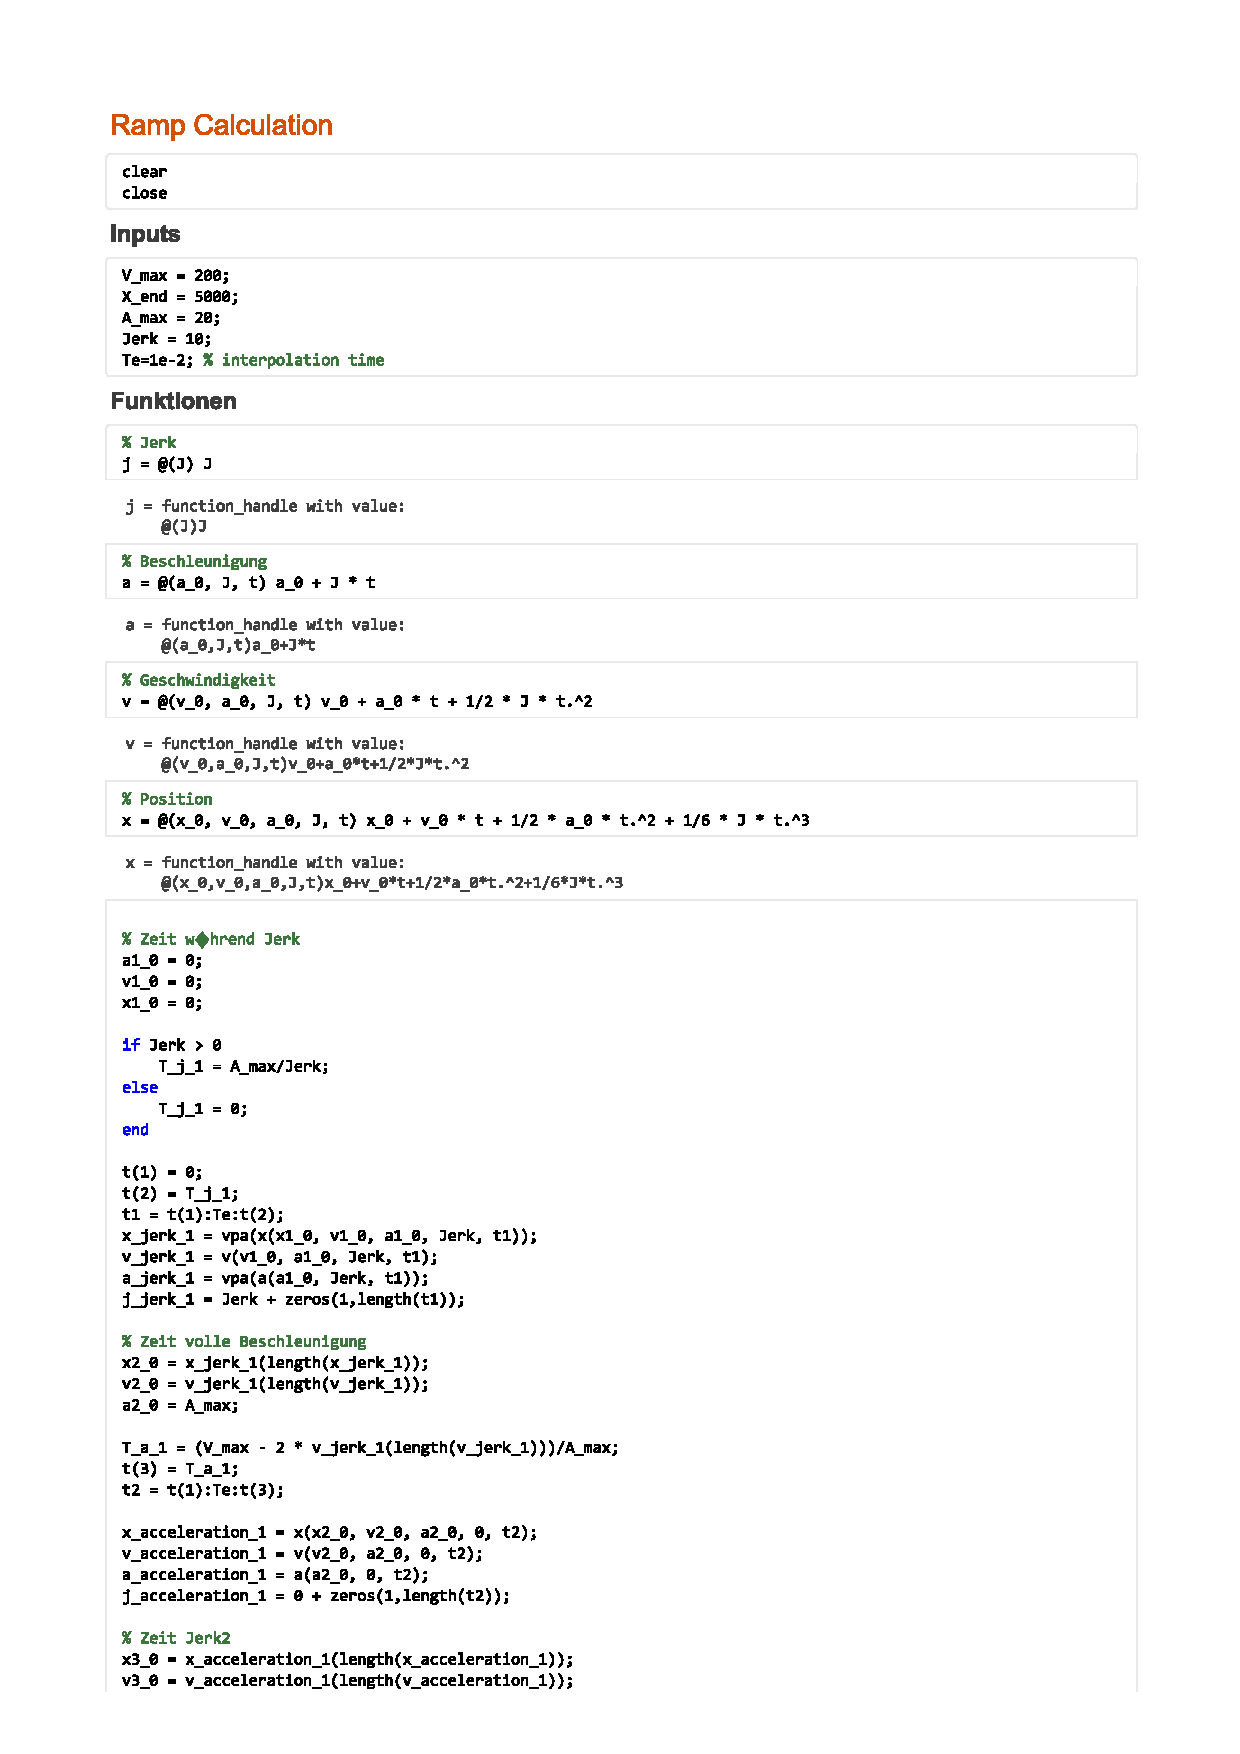
\includepdf[pages={1}]{appendix/Ramp_Script}
\includepdf[pages={2}]{appendix/Ramp_Script}
\includepdf[pages={3}]{appendix/Ramp_Script}
